\documentclass[12pt,one column]{article}
\usepackage{listings}
\usepackage{float}
\usepackage{mathtools}
\usepackage[english,russian]{babel}
\everymath{\displaystyle}
\usepackage{hyperref}
\usepackage[usenames]{color}
\usepackage{colortbl}
\usepackage{booktabs}
\usepackage{placeins}
\usepackage{longtable}
\usepackage{multirow}
\usepackage{xcolor}
\usepackage{verbatim}
\usepackage[T2A]{fontenc}
\usepackage{geometry}
\geometry{
  a4paper,
  top=25mm, 
  right=15mm, 
  bottom=25mm, 
  left=15mm
}

\begin{document}
\begin{center}
    Санкт-Петербургский Национальный Исследовательский\\ 
    Университет ИТМО\\
    Мегафакультет Компьютерных Технологий и Управления\\
    Факультет Программной Инженерии и Компьютерной Техники \\
    
\includegraphics[scale=0.2]{itm.jpg} % нужно закинуть картинку логтипа в папку с отчетом
\end{center}
\vspace{1cm}


\begin{center}
    \large \textbf{Вариант №P3210173}\\
    \textbf{Лабораторная работа №4}\\
    по дисциплине\\
    \textbf{Веб-программирование}
\end{center}

\vspace{2cm}

\begin{flushright}
  Выполнил Студент  группы P32101\\
  \textbf{Лапин Алексей Александрович}\\
  Преподаватель: \\
  \textbf{Пашнин Александр Денисович}\\
\end{flushright}

\vspace{6cm}
\begin{center}
    г. Санкт-Петербург\\
    2022г.
\end{center}
\newpage
\tableofcontents
\newpage
\section{Текст задания:}
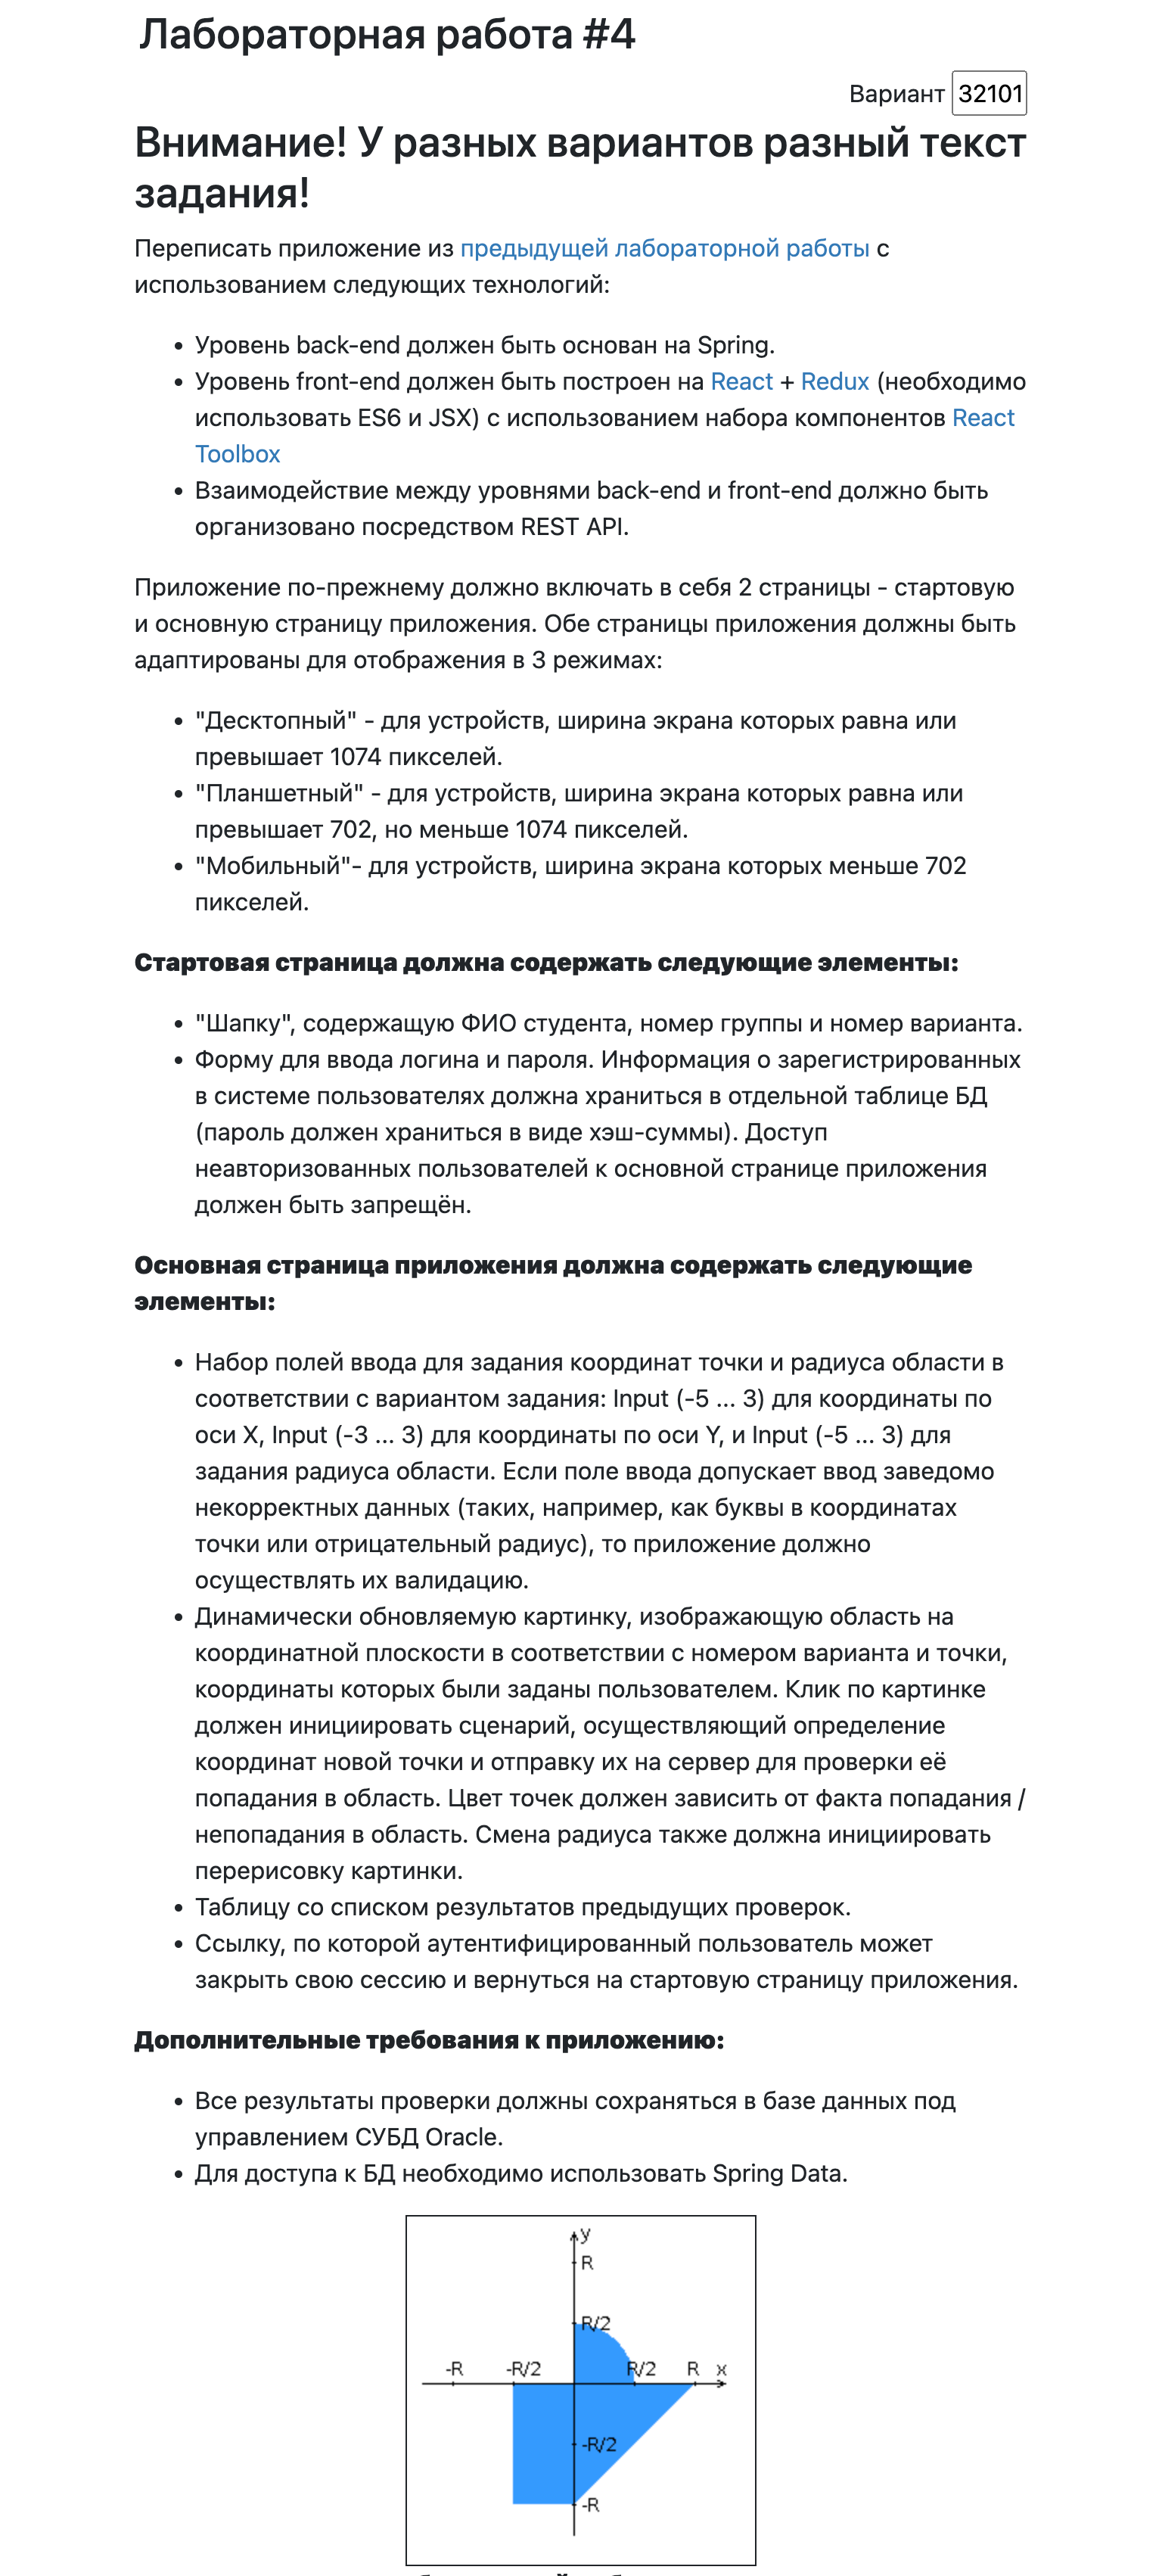
\includegraphics[width=0.55\textwidth]{Task.png}
\section{Код}
frontend: 
\href{https://github.com/AaLexUser/web-4-frontend}{https://github.com/AaLexUser/web-4-frontend}\\
backend: \href{https://github.com/AaLexUser/web-4}{https://github.com/AaLexUser/web-4}
\section{Вывод программы}
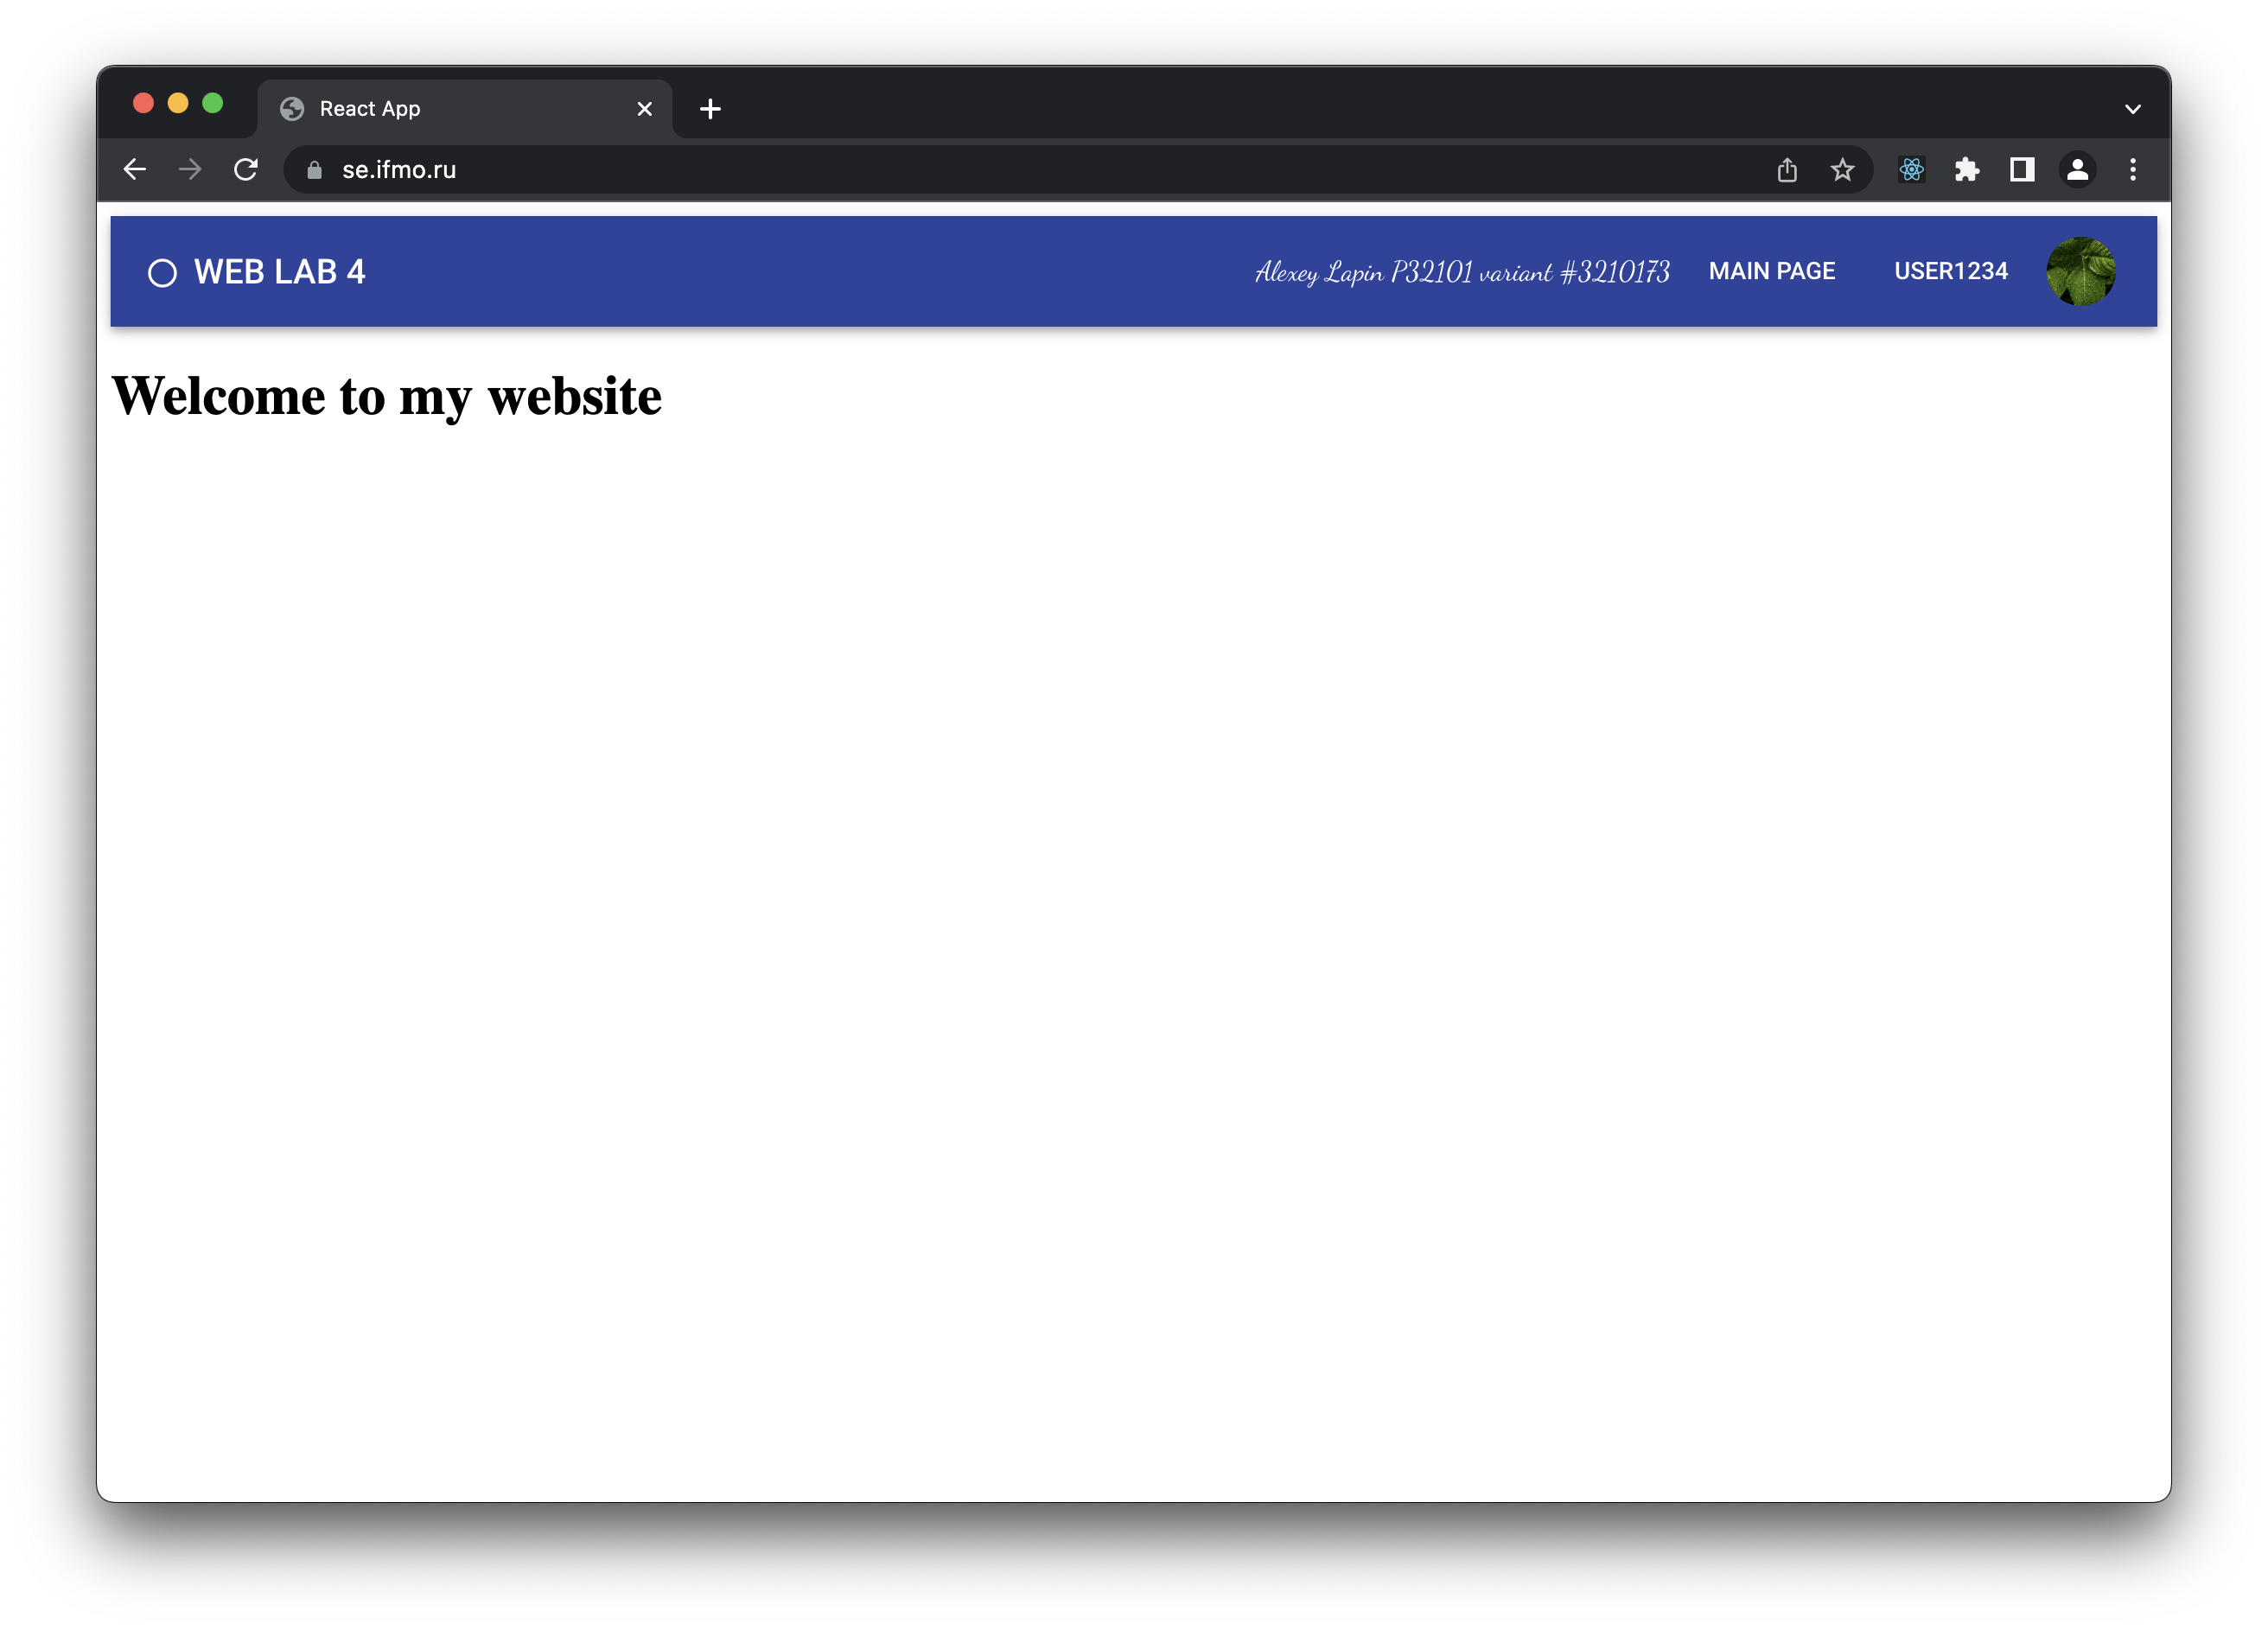
\includegraphics[width=\textwidth]{prog1.png}
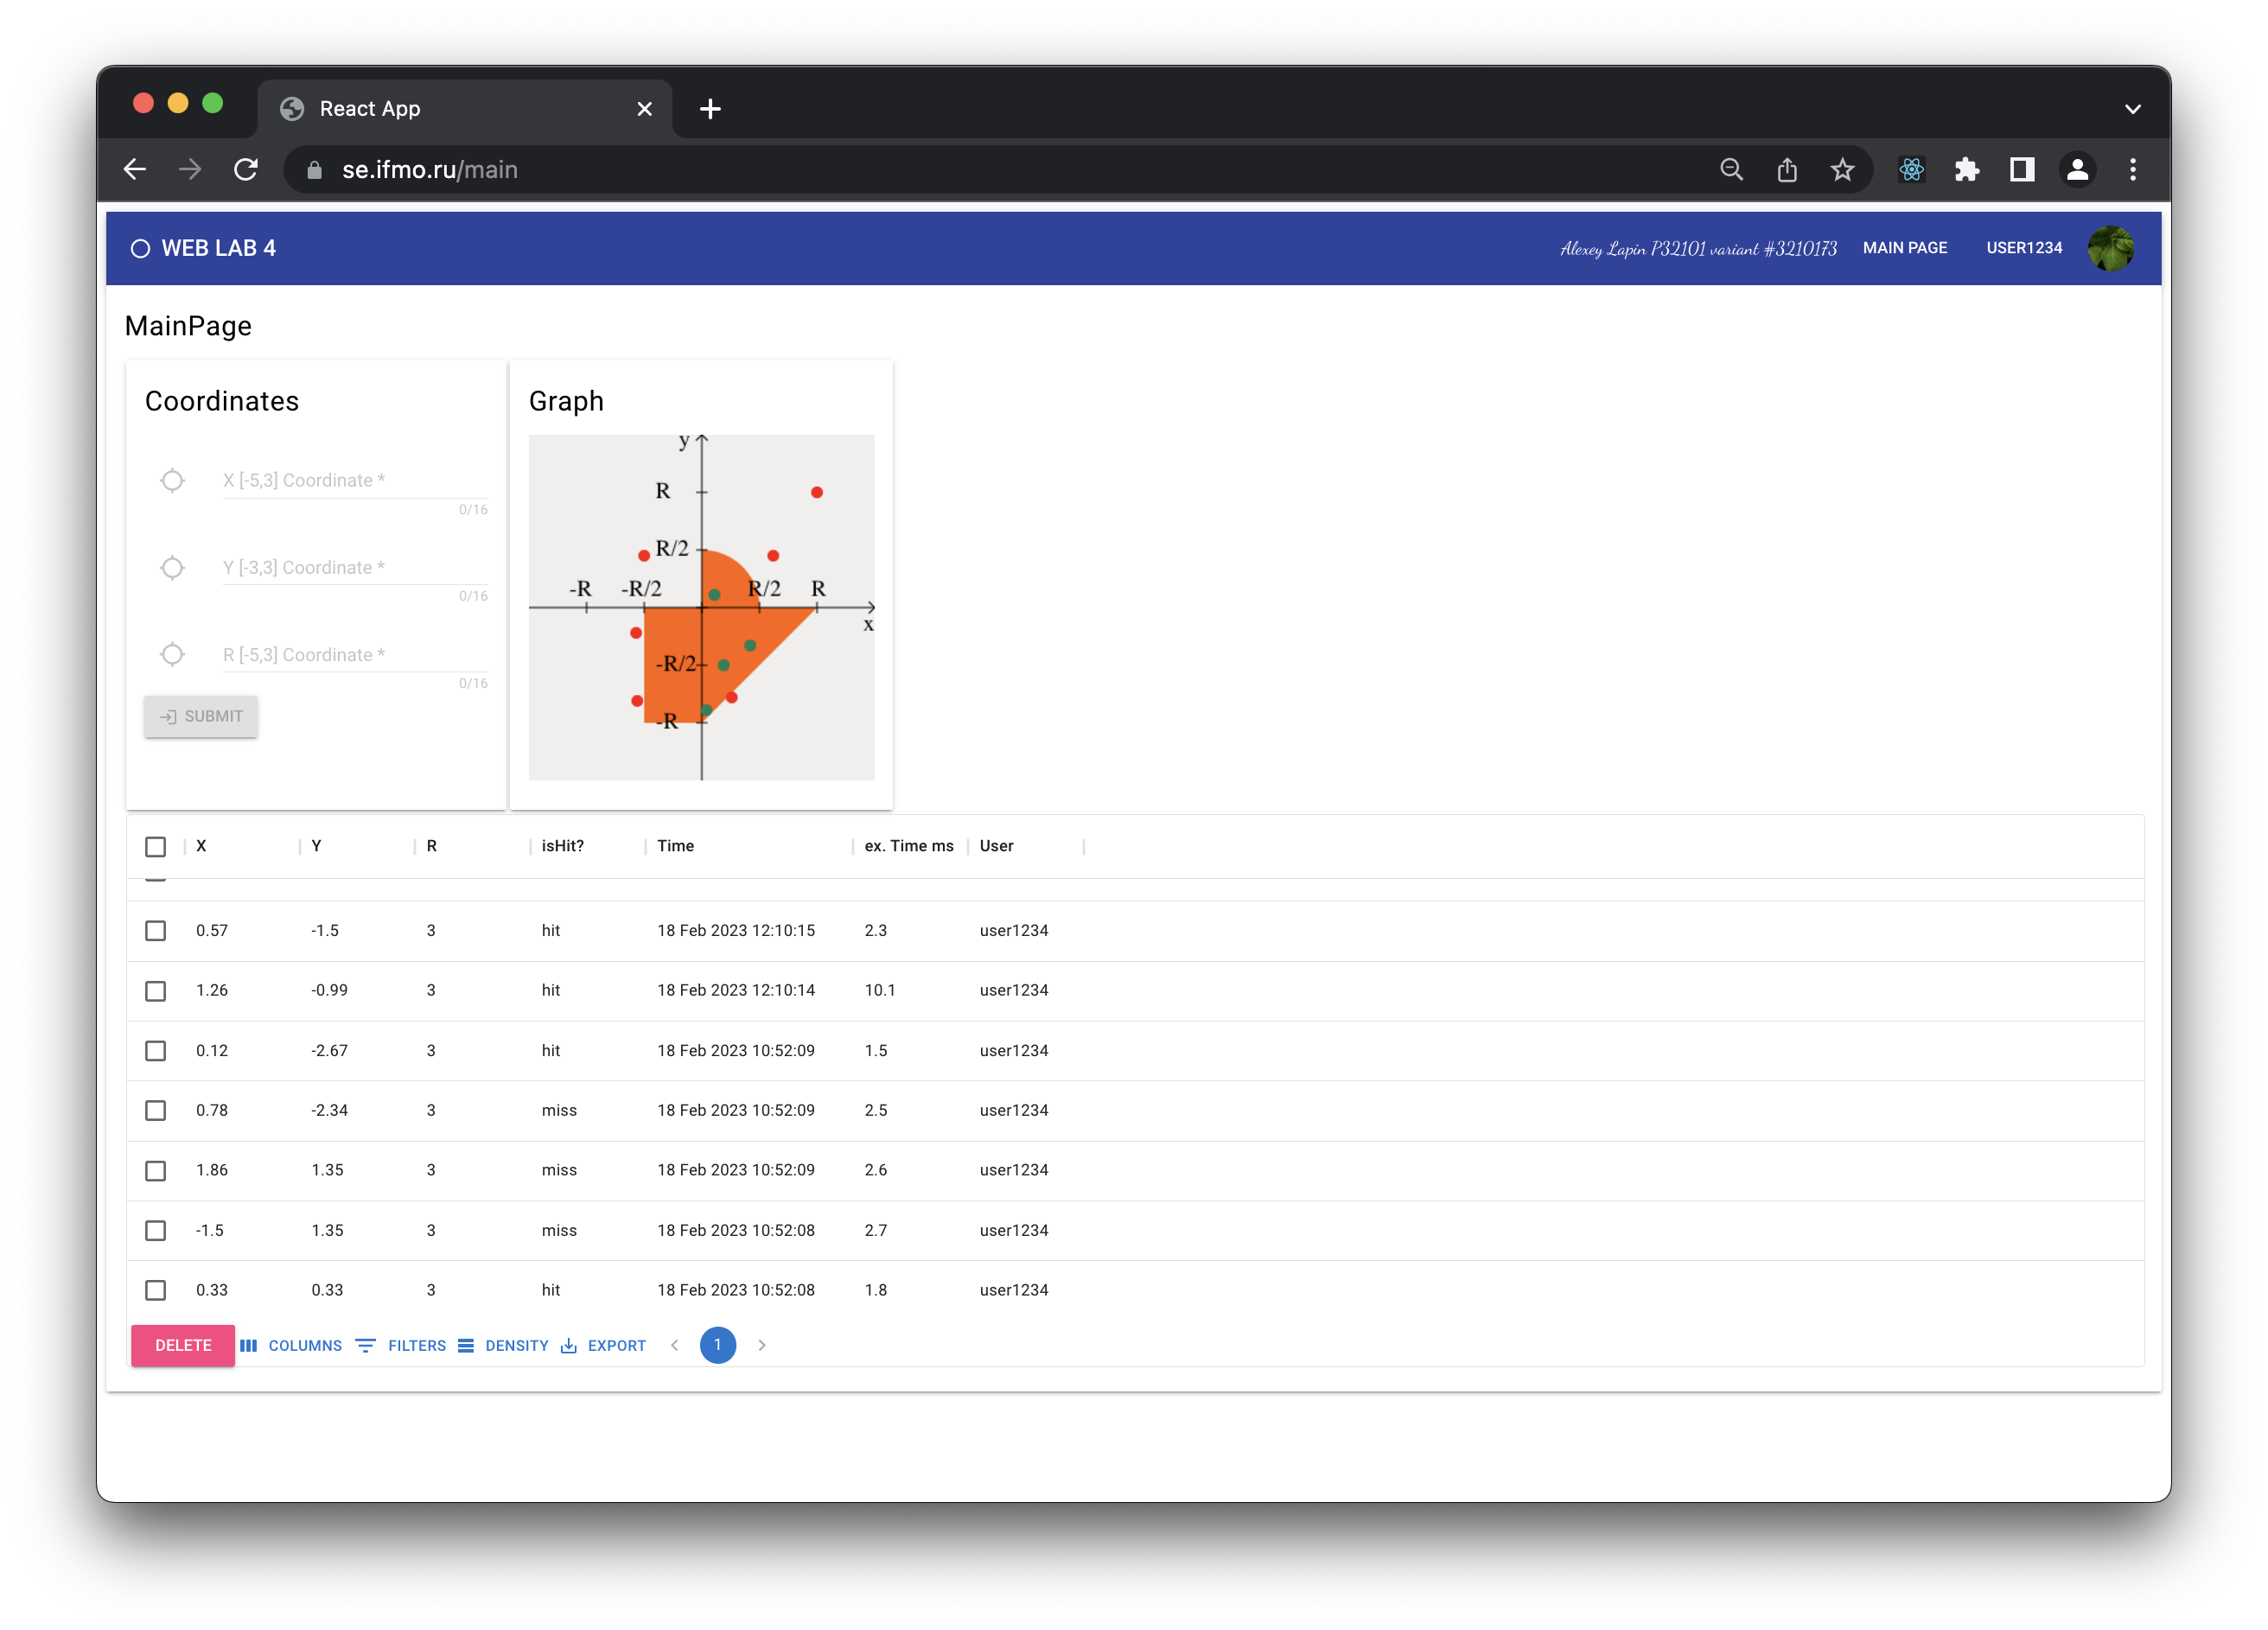
\includegraphics[width=\textwidth]{prog2.png}
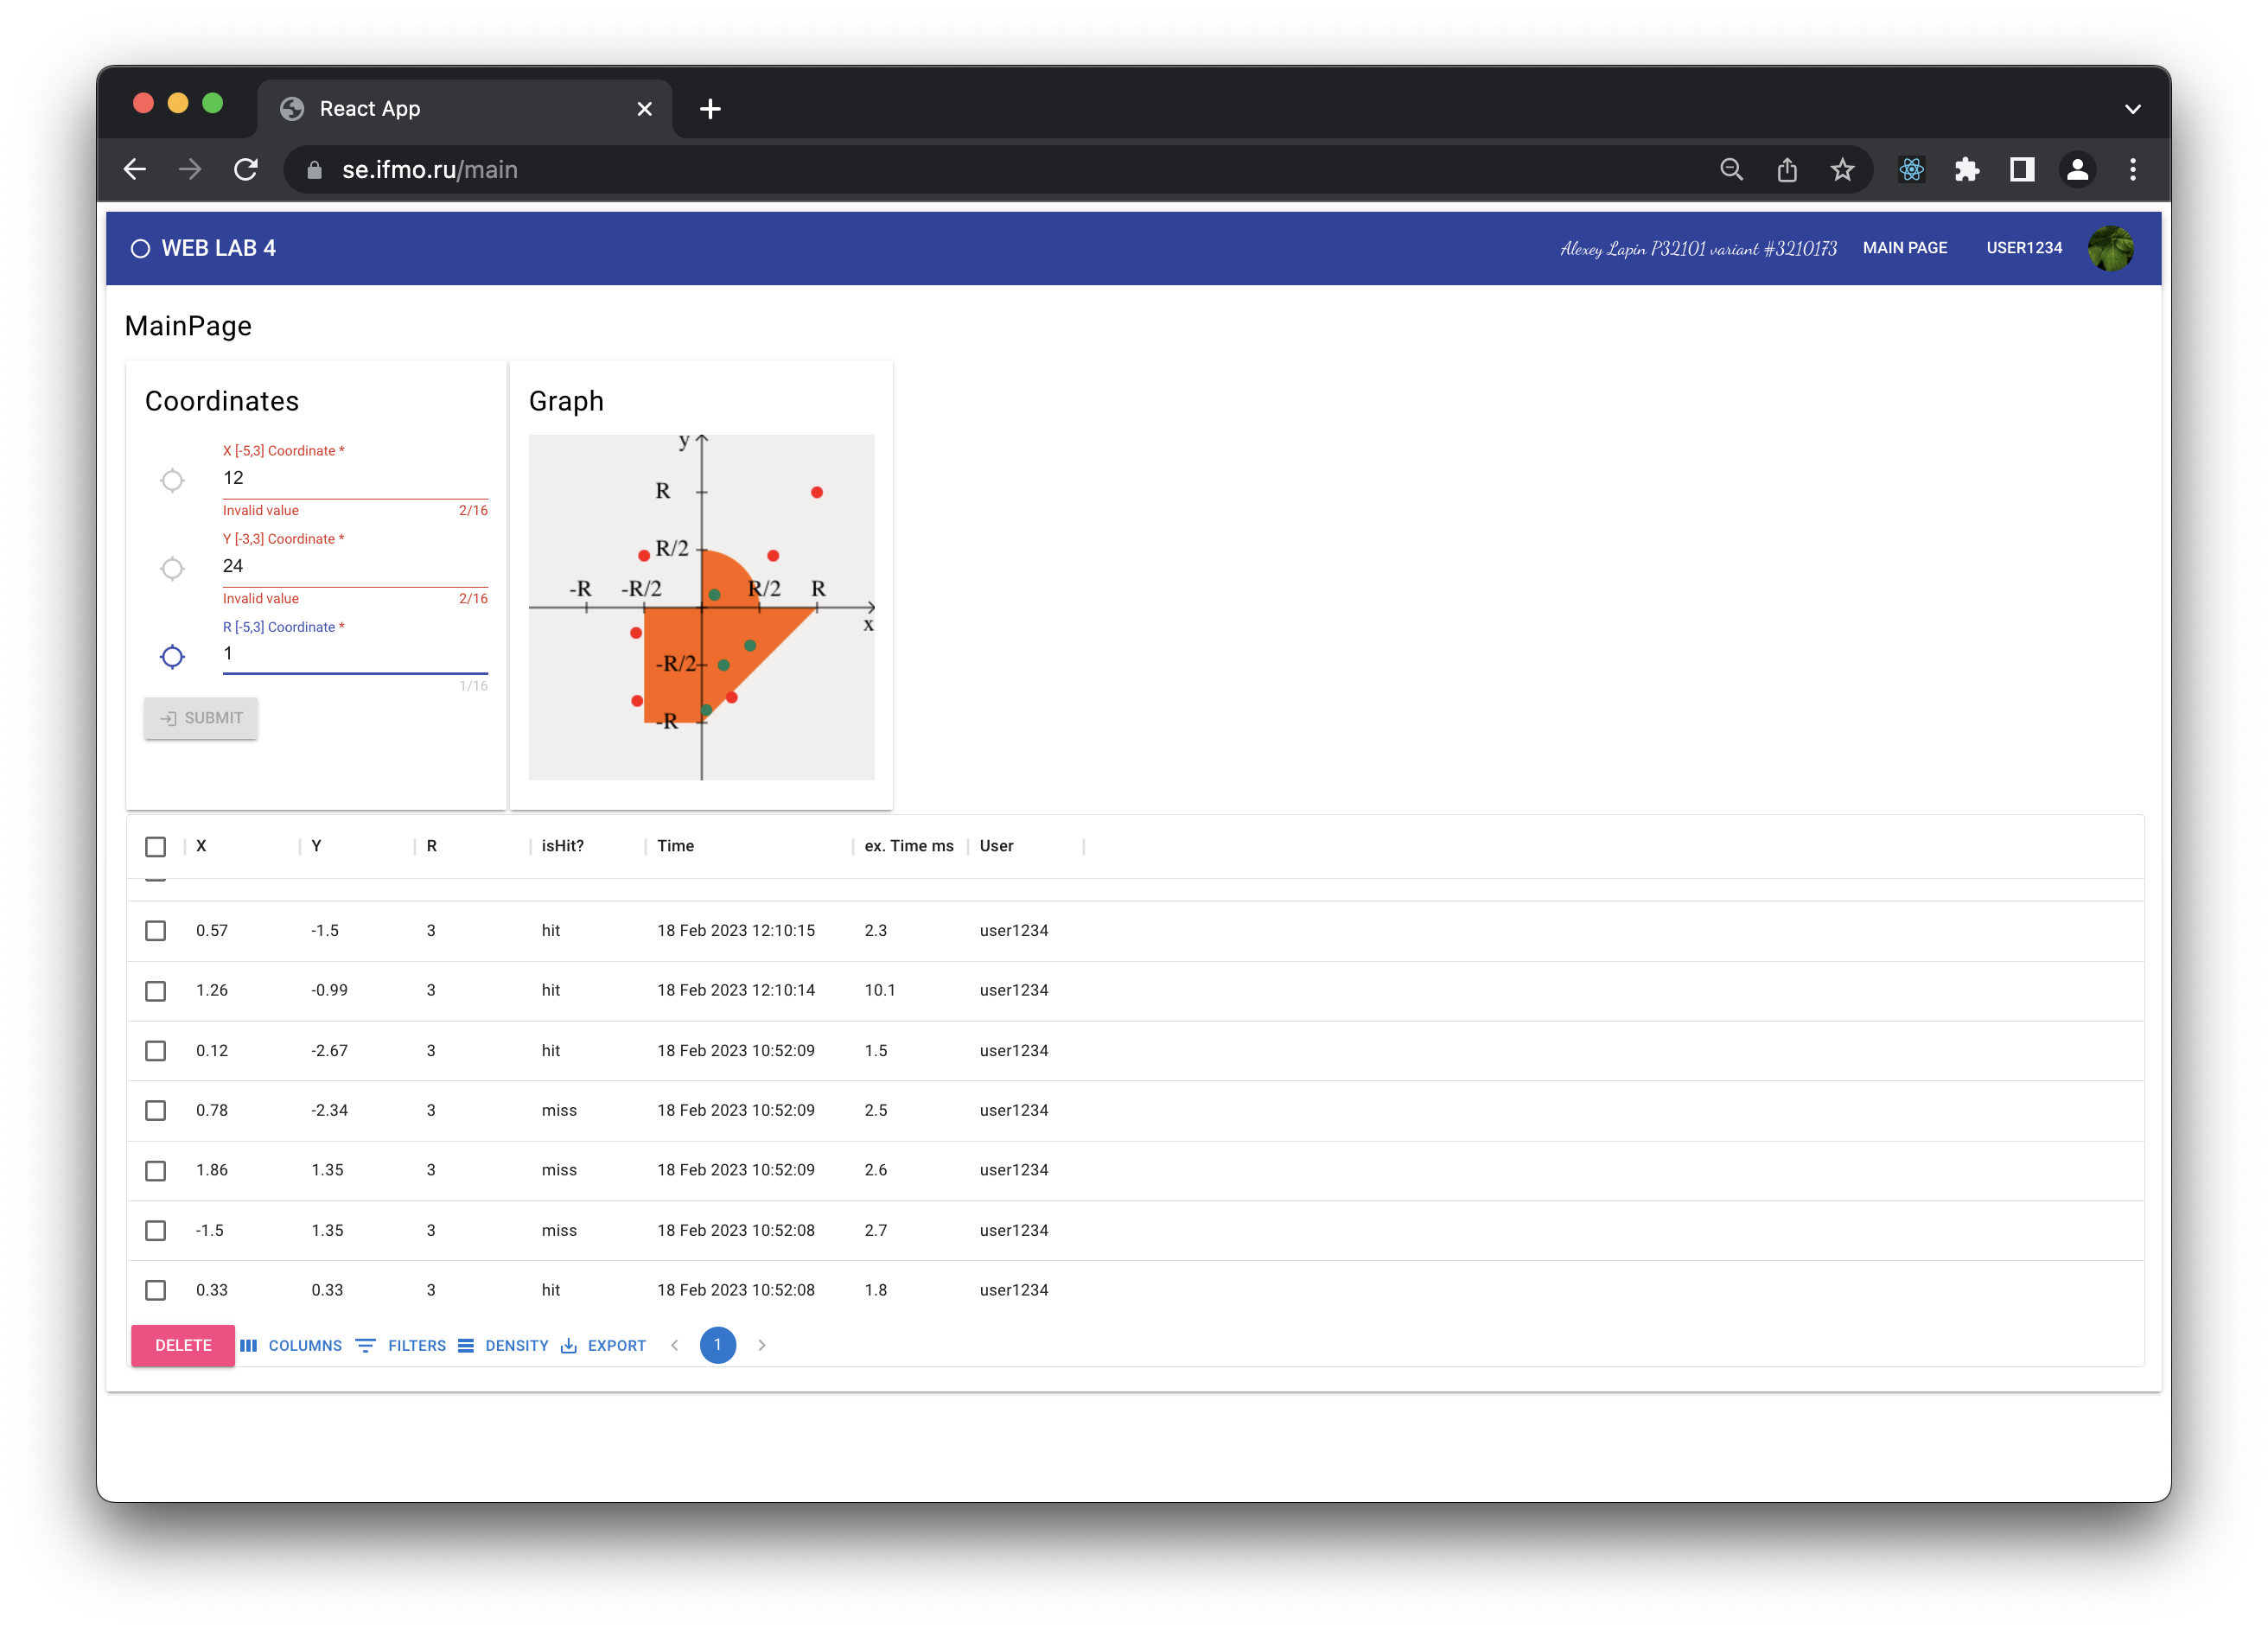
\includegraphics[width=\textwidth]{prog3.png}
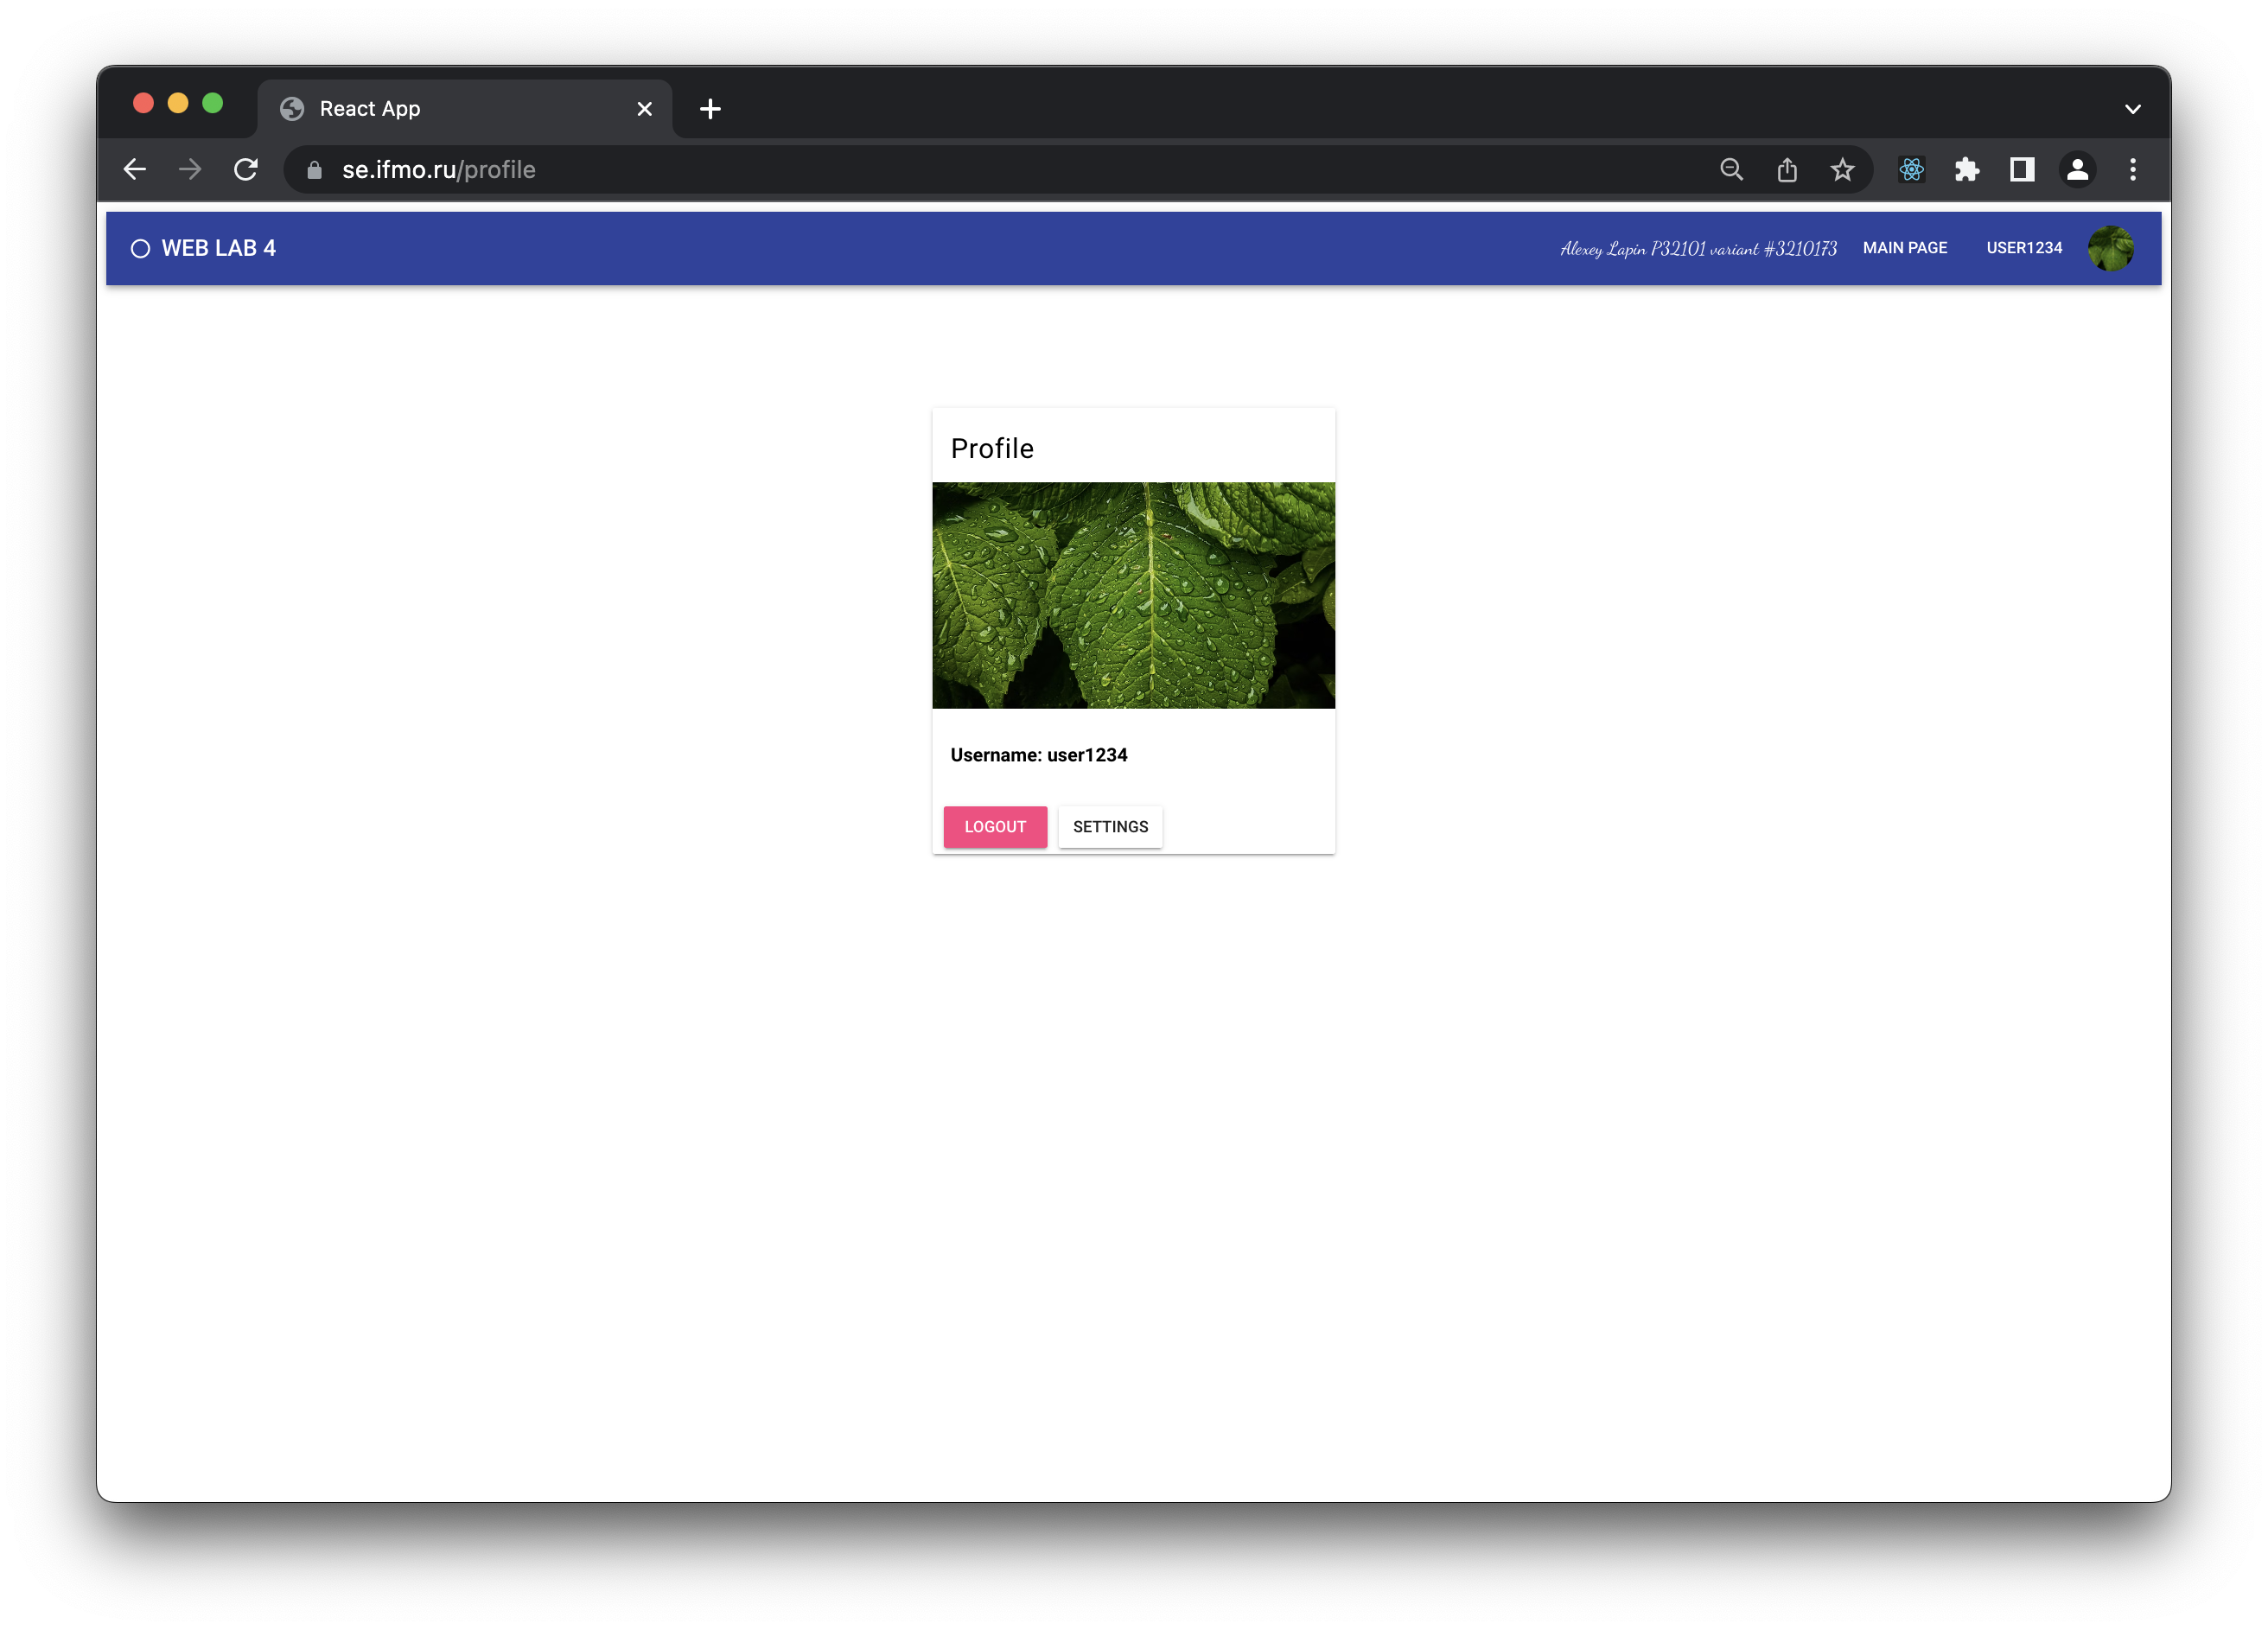
\includegraphics[width=\textwidth]{prog4.png}
\section{Вывод:}
В этой лабораторной работе я познакомился с:
\begin{enumerate}
    \item React
    \item Redux
    \item TypeScript
    \item Java Spring
\end{enumerate}
\end{document}